\subsection{拓扑空间的克鲁尔维数}

定义 1. --- 设 I 是一个有序集。I 的一个非空有限全序子集称为 I 的一条链。设 c 是 I 的一条链；c 的最小元和最大元称为 c 的端点。整数 Card(c) - 1 称为 c 的长度。I 的子集集合上的包含关系在 I 的链集合上诱导出一个序关系。如果 I 中具有与 c 相同端点的链里 c 是极大的，则称链 c 是饱和的。

为了表示长度为 n 的链，我们常写作“链” \(i_{0} < \cdots < i_{n}\)，其中 \(i_{k}\) 是 c 的元素，并按从 0 到 n 的整数严格递增地编号。

设 X 是一个拓扑空间。我们在 X 的不可约闭子集集合（II, § 4, no. 1, def. 1）上赋予由包含关系定义的序关系。当我们说 X 的不可约闭子集的一条链时，始终指按此序关系的一条链。

定义 2. --- 我们称拓扑空间 X 的克鲁尔维数为 dim kr(X)，或简单记为 dim(X)，即 X 的不可约闭子集的链长集合在 \(\overline{\mathbf{R}}\) 中的上确界。

对于 X 中的每个点 x，我们称 \(\dim_{x}(X)\) 为 X 在 x 处的克鲁尔维数；它是 x 的开邻域的维数的下确界。

我们有 \(\dim(\emptyset) = -\infty\) 。另一方面，如果 X 非空，则 X 中任一点的闭包都是 X 的不可约闭子集（II, § 4, no. 1, prop. 2），因而 X 的维数或者是 +∞，或者是一个正整数。假设 X 是分离的且非空；那么 X 的每个不可约子集都退化为一点，且 X 的维数为 0。

\pandocbounded{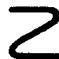
\includegraphics[keepaspectratio]{images/part001_0d60a61e.jpg}}

因此，对于分离空间，克鲁尔维数的定义没有什么意义，但它特别适合交换代数中遇到的拓扑空间（环的谱、*概形*、\ldots）。在本章中，不会与拓扑空间的其他维数概念（例如勒贝格维数）混淆，我们将简单地用“维数”表示“克鲁尔维数”。

命题 1. --- 设 X 是一个拓扑空间。

\begin{enumerate}
\def\labelenumi{\alph{enumi})}
\item
  如果 Y 是 X 的子空间，则有 \(\dim(\mathbf{Y}) \leqslant \dim(\mathbf{X})\)，且有 \(\dim_y(\mathbf{Y}) \leqslant \dim_y(\mathbf{X})\) 对 Y 的每个点 \(y\) 都成立。
\item
  设 \(x\) 是 \(X\) 的一个点，\(V\) 是 \(x\) 在 \(X\) 中的一个邻域。我们有 \(\dim_x(X) = \dim_x(V)\)。
\item
  设 \((\mathbf{X}_i)_{i\in I}\) 是 X 的闭子集的一个有限族，使得 \(\mathbf{X} = \bigcup_{i\in I}\mathbf{X}_i\)。我们有
\end{enumerate}

\(\dim(X) = \sup_{i \in I} \dim(X_i)\)且，对于每个点 \(x\)（属于 \(X\)），有 \(\dim_x(X) = \sup_{i \in J_x} \dim_x(X_i)\)，其中 \(J\) 表示满足 \(i \in J\) 且 \(x \in X\) 的指标集合。

其中  表示满足  的  的集合。\[
\mathrm{J} _ {x}
\]

证明 a)。如果 Z 是 Y 的不可约闭子集，则它在 X 中的闭包 \(\overline{Z}\) 是不可约的（II, § 4, no. 1, prop. 2），且有 \(\overline{Z} \cap Y = Z\)。因此，Y 的每条不可约闭子集链 \(c\) 通过在 X 中取闭包，定义了 X 的一条不可约闭子集链，其长度与 \(c\) 相同。由此得到不等式 \(\dim(Y) \leqslant \dim(X)\)。如果 U 是 X 中包含 Y 的一个点 \(y\) 的开子集，则有 \(\dim(U \cap Y) \leqslant \dim(U)\)，从而 \(\dim_y(Y) \leqslant \dim_y(X)\)。

证明 \(b\)。按定义 \(\dim_{x}(X) \leqslant \dim_{x}(V)\)，反向不等式由 \(a\)）得出。

证明 \(c\)。设 \(Z_{0} \subset \ldots \subset Z_{n}\) 是 X 的不可约闭子集的一条链。我们有 \(Z_{n} = \bigcup_{i \in I} (Z_{n} \cap X_{i})\)，且每个集合 \(Z_{n} \cap X_{i}\) 都在 \(Z_{n}\) 中闭；

由于 I 有限，\(Z_{n}\) 包含于某个 \(X_{i}\) 中。因此有 \(\dim(X) \leqslant \sup_{i} \dim(X_{i})\)，由 \(a\)）即得等式。

现在设 \(x\) 是 \(X\) 的一个点，且 \(n = \sup_{i \in J_x} \dim_x(X_i)\)，其中 \(J_x\) 如命题中所述。由 \(\dim_x(X) \geqslant n\) \(a\)）；为证明等式，不妨设 \(n\) 有限。对每个 \(i \in J_x\)，取 \(U_i\) 为 \(x\) 在 \(X\) 中的一个开邻域，使得 \(\dim(U_i \cap X_i) \leqslant n\)。置 \(U = (\bigcap_{i \in J_x} U_i) \cap (\bigcap_{i \in I - J_x} \complement X_i)\)；集合 \(U\) 在 \(X\) 中是开集。此外，由上一段有 \(\dim(U) = \sup_{i \in J_x} \dim(U \cap X_i) \leqslant n\)，从而 \(\dim_x(X) \leqslant n\)。

推论。--- a) 拓扑空间 X 的维数是其不可约分支的维数的上确界（II, § 4, no. 1, definition 2）。

\begin{enumerate}
\def\labelenumi{\alph{enumi})}
\setcounter{enumi}{1}
\tightlist
\item
  设 \(x\) 是 \(X\) 的一个点。我们有 \(\dim_x(X) \geqslant \sup_i \dim_x(X_i)\)，其中 \(X_i\) 遍历族。
\end{enumerate}
包含 x 的 X 的不可约分支族；如果 x 有一个仅含有限个不可约分支的邻域 V，则有等式（例如 V 为诺特空间时就是如此）。


第一条断言是直接的，因为 X 的不可约闭子集链正是 X 的不可约分支的不可约闭子集链（II, § 4, no. 1, prop. 5）。不等式 \(\dim_x(X) \geqslant \sup_i \dim_x(X_i)\) 由

命题 1 a) 得出。设 V 是 x 的一个仅含有限个不可约分支的邻域，令 \((\mathrm{V}_{j})_{j\in\mathbb{J}}\) 为包含 x 的 V 的不可约分支族。由命题 1 b) 和 c) 可得

\[
\dim_ {x} (X) = \dim_ {x} (V) = \sup _ {j \in J} \dim_ {x} (V _ {j});
\]

我们只需注意，每个 \(V_{j}\) 都包含于某个 \(X_{i}, i \in J_{x}\)，因而有 \(\sup_{j \in J} \dim_{x}(V_{j}) \leqslant \sup_{i \in J_{x}} \dim_{x}(X_{i})\)，于是得到结论。

命题 2. — 设 X 是一个拓扑空间。我们有 \(\dim(X) = \sup_{x \in X} \dim_x(X)\)。

事实上，按定义，有 \(\dim(X) \geqslant \dim_x(X)\) 对每个 \(x \in X\) 都成立。另一方面，如果 \(Z_0 \subset \ldots \subset Z_n\) 是 \(X\) 的不可约闭子集链，则对所有 \(x \in Z_0\) 以及 \(U\)（\(x\) 的每个开邻域），集合 \(Z_0 \cap U, \ldots, Z_n \cap U\) 构成 \(U\) 的不可约闭子集链（II, § 4, no. 1, prop. 7）。因此有 \(\dim_x(X) \geqslant n\)，从而 \(\dim(X) \leqslant \sup_{x \in X} \dim_x(X)\)。

推论。— 如果 \((\mathrm{X}_{\alpha})_{\alpha\in\mathbf{A}}\) 是拓扑空间 X 的一个开覆盖或局部有限闭覆盖，则有

\[
\dim (X) = \sup _ {\alpha \in A} \dim (X _ {\alpha}).
\]

只需证明，对于每个点 \(x\)（属于 \(X\)），有 \(\dim_x(X) = \sup_{\alpha \in A_x} \dim_x(X_\alpha)\)，其中 \(A_x\) 是由满足 \(\alpha \in A\) 且 \(x \in X_\alpha\) 的指标组成的集合。开覆盖的情形显然；局部有限闭覆盖的情形则由命题 1 c) 得出。

